\documentclass[12pt]{article}
\usepackage{geometry}
\geometry{a4paper, total={170mm,257mm},left=20mm, top=20mm,}
\usepackage[colorlinks=true,linkcolor=blue,urlcolor=black]{hyperref}
\usepackage{bookmark}
\usepackage{listings}
\usepackage{enumitem}
\usepackage[autostyle, english = american]{csquotes}
\usepackage{courier}
\usepackage{graphicx}
\usepackage{mdframed}
\begin{document}
\begin{titlepage}
\centering
\vfill
\vspace*{4\baselineskip}
{\bfseries\Large
Labtainer Framework Development Guide\par
}
\vspace*{4\baselineskip}
{\bfseries
Fully provisioned cybersecurity labs\par
}
\vspace*{2\baselineskip}
\today
\vfill
%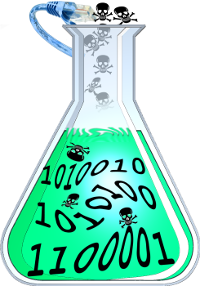
\includegraphics[natwidth=200, natheight=286]{labtainer5-sm.png}
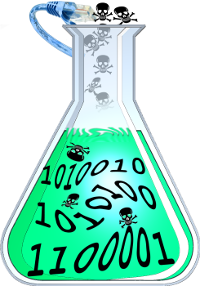
\includegraphics[width=0.4\textwidth]{labtainer5-sm.png}
\vfill

\vspace{2.0in}
This document was created by United States Government employees at 
The Center for Cybersecurity and Cyber Operations (C3O) at the Naval Postgraduate School NPS. 
Please note that within the United States, copyright protection is not available for any works created  
by United States Government employees, pursuant to Title 17 United States Code Section 105.   
This document is in the public domain and is not subject to copyright. 
\end{titlepage}
\tableofcontents
\newpage
\section {Introduction}
This document is intended for use by developers who maintain the
Labtainer framework.  It is also applicable to lab designers who wish
to follow Labtainers configuration management and testing conventions for  their labs.
It does not address the mechanics of lab creation, which are 
covered in the \textit {Labtainers Lab Designer User Guide}.

\begin{flushleft} 
{\bf Note:} 
The Labtainer framework is developed within and for Linux environments using the command line.
\end{flushleft} 

The procedures described herein assume development occurs on a Linux VM that itself is hosted on
a Linux platform using VirtualBox.  That underlying Linux platform also hosts \textit{test VMs} that
will run regression tests.  Other configurations are certainly possible, but they would require the
developer to potentially alter procedures and/or scripts.

The VirtualBox product is used to to run Labtainer VMs for testing.  Currently, tests are performed on 
Ubuntu16 and Ubuntu18 VMs, the former tests backwards compatibility of the frameworks python3 support.


\subsection{Linux host installation}
The host platform should include VirtualBox (to host the Development VM and test VMs),  and Docker, 
(to host a set of test registries).  The host platform should have a directory named SEED that will
be shared by each of the VMs.  If the host is to publish distributions to the NPS website, then it should
have an ability to transfer files to 
\begin{verbatim}
davs://nps.edu/webdav/c3o-staging/document_library/labtainers
\end{verbatim}

\section{Development VM Installation}
This section describes installation of software on the development VM, which should have at least 150 GB
of disk.
\subsection{Developer Software Prerequisites}
Labtainers is primarily implemented using python3.  The containers within a lab include python2 scripts that are
part of the framework, e.g., functions that collect student artifacts.  The following packages are required on a
Linux distribution to support Labtainer framework development.  The packages can be installed using the
{\tt setup\_scripts/dev-pkg.sh} script.

\begin {itemize}
\item {\bf git}
\item {\bf make}
\item {\bf g++}
\item {\bf Latex} (texlive-latex-base and texlive-latex-extra)
\item {\bf Docker (Community Edition)} [See {\bf Docker Installation} Section \ref{docker-install}]
\item {\bf pip3} {\tt apt-get install python3-pip}
\item {\bf dateutil} {\tt pip3 install py-dateutil}
\item {\bf xdotool} 
\end {itemize}

\subsection{Getting Labtainers from Github}

In a Linux terminal, change the working directory into the directory you want to store Labtainers.
\begin{flushleft} Run this in the terminal: \end{flushleft}
\begin{center} {\tt git clone https://github.com/mfthomps/Labtainers.git} \end{center} 

\subsection{Setting up the Development Environment}
\begin {itemize}
\item Disable any auto-updates on your machine as this may interfere with 'apt-get' requests you may have during development.
\item Modify your ~/.bashrc file.
    \begin{enumerate}
    \item Add {\bf LABTAINER\_DIR} as an environment variable and set its value as the path to the {\tt  /Labtainers} directory. 
    \item Modify the \$PATH to include {\tt ./bin} and {\tt \$LABTAINER\_DIR/scripts/designer/bin}.
    \item In summary, your ~/.bashrc should include something like this:
	    \lstset{basicstyle=\footnotesize\ttfamily,
		    breaklines=true
	    	    framextopmargin=50pt
		    frame=single,
		    language=bash}
	    \begin{mdframed}
	    \begin{lstlisting}
export LABTAINER_DIR=$HOME/Labtainers
export TEST_REGISTRY="YES"
if [[ ":$PATH:" != *":./bin:"* ]]; then
  export PATH="${PATH}:./bin:$LABTAINER_DIR/scripts/designer/bin"
fi
	    \end{lstlisting}
	    \end{mdframed}
    \end{enumerate}
\item cd into \$LABTAINER\_DIR/setup\_scripts:
    \begin{itemize}
    	\item Run build-docs.sh to build the lab manuals for all labs.
    \end{itemize}
\item cd into \$LABTAINER\_DIR/tool-src/capinout and run {\tt ./mkit.sh}
\item Add the vbox share group using {\tt setup\_scripts/vbox-share.sh} 
\item Map the SEED directory on the Linux host as a shared folder. This directory is used
to share distribution files between the development system and the test VMs.  Accept defaults so its name is 
\begin{verbatim}
        /media/sf_SEED
\end{verbatim}
\end {itemize}


\subsection{Docker Installation}
\label{docker-install}
For full and convenient installation of Docker and setting of Docker privileges, run  'install-docker-ubuntu.sh' in 'setup\_scripts', assuming you are developing in Ubuntu. {\bf Note:} Make sure to run the script as user (not sudo), so that your user can be added to the Docker group.\\ 
    

    \begin {itemize}
    \item If on a different Linux distribution look in the same folder for your corresponding distribution (CentOS, Debian, Fedora). 
    \item If your Linux distribution is none of these, please view Docker's webpage documentation to learn how to install Docker and set Docker privileges on your machine.
    \item {\bf NOTE:} These install-docker scripts include the installation of other packages outside Docker that are necessary for building labs. 
    \end {itemize}

\noindent Reboot the system, so that user receives Docker privileges.

\noindent Run pull-all.py to get all base docker images.


\section {Framework implementation overview}
\subsection{Implementation elements}
The Labtainer framework implementation is primarily python scripts.  A number of the 
top level scripts share functions found in scripts/labtainer-student/{\bf bin}/labutils.py.  The 
top level scripts are organized as follows:

\begin{itemize}
	\item {\bf Student} \begin{itemize}
\item {\tt labtainer} (start) and {\tt stoplab} -- In the labtainers-student/bin directory, these run on the 
Linux host and manage the pulling, starting and stopping of containers.  They also coordinate
collection of student artifacts.
\item Container scripts -- In the labtainers-student/{\bf lab\_bin} directory, these execute on
containers, e.g., to hook bash and parameterize containers.
	\end{itemize}

	\item {\bf Instructor} \begin{itemize}
\item {\tt gradelab} and {\tt stopgrader}-- Push student artifacts onto grader container and get assessment results.
\item Container scripts -- perform grading functions.
\item Web interface -- The {\tt -w} option to gradelab starts a Flask web server on the container, found in the
{\tt flask/server.py}.  When debugging and enhancing this, use the {\tt -v} option instead of the {\tt -w} option to
cause the development flask directory to be mounted by the container.  Then start the server with {\tt .local/flask/server.py labname}.
	\end{itemize}

	\item {\bf Lab designer} \begin{itemize}
\item Building -- rebuild in labtainers-student/bin 
\item Publishing labs -- labtainers/distrib/publish.py
\item Base Labtainer images -- scripts/designer/bin, create and publish the base images.
	\end{itemize}	

	\item {\bf Other} \begin{itemize}
\item VM appliances -- //host\_scripts, update and publish VM appliances as OVA files for 
VirtualBox and VMWare.
\item Regression testing of grading functions is performed by labtainer-instructor/regress.py.
Expected results are stored in the labtainer/testsets directory.
\item Regression testing of labs and grading combined: scripts in testsets/bin; data sets
are not distributed, they are in {\tt labtainer/simlab/<labname>}  Get simlab data sets using
\begin{verbatim}
git clone https://gitlab.nps.edu/mfthomps/Labtainers-simlab.git/
\end{verbatim}

       \end{itemize}

\end{itemize}

\subsection{Control flow}
Student scripts, e.g., {\tt labtainer}, run from the scripts/labtainer-student directory.
That directory also contains the bin/labutils.py, which contains most of the framework
functions.

The first time a given lab is run, the {\tt docker create} function is
used to create containers.  The {\tt docker start} function is then used to start
the container, and is used for subsequent starts of the same lab.

When a student container is first started "docker exec" is used
to run parameterize.sh on the container.

That script also invokes hookBash.sh, which adds the bash
sdtin/stout capturing hook, and adds the startup.sh call
into the .profile.

The startup.sh uses a lock to control which
terminal displays the instructions.  In practice most
instructions are now pdf files.
The startup.sh invoked by student will source a student\_startup.sh if present.

The Student.py script runs when a lab is stopped to collect artifacts and kill lingering
monitored processes.

Grading is performed on a separate container built for each lab, derived from the 
labtainer.grader image.

The {\tt checkwork} function forces a collection of artifacts, and a grader container
is then run to perform grading.

\subsection{mynotify}
The mynotify runs as a service.  It is installed from the labtainer-student/lab\_bin directory.
It will exit silently if the lab has no notify file in .local/bin.  See its log on each container
within /tmp/mynotify.log  The service uses the Linux inotify service to detect and record access to files.

\section{Distribution publishing}
The Labtainer framework is distributed via the c3o website as a tar file, or, optionally a
VM applicance (both VMWare and VirtualBox).  The Docker images are distributed via the Docker Hub.

The labtainer/distrib/mkdist.sh script runs on a Linux VM hosted on windows or Linux, and creates the distribution tar 
and copies it into a shared folder.  The mk-devel.sh script makes the developers version of the tar.
From that shared folder, the two tar files are copied to the 
\begin{verbatim}
\\my.nps.edu@SSL\DavWWWRoot\webdav\c30-staging\document\_library" 
\end{verbatim}
\noindent and then "Publish to Live" is 
performed on the Liferay site.

The distributions are created from a git repos, as described in section \ref{releases}.

\subsection{VM Appliances}
Two prepackaged VM appliances are maintained: one for VirtualBox, and one for VMWare.  Each include
their respective guest additions.  The VMs are maintained on a native Linux system using command line
utilities, e.g., VBoxManage.  The VMs are rigged to update Labtainers, including a pull of
baseline images, on each boot until the first lab is commenced.  Scripts named "export*" are
used to created the appliance files.  The scripts re-import into test images, which must be
manually tested.  The WinSCP script pushes new applicance images to the CyberCIEGE download
directory on the C3O web server.  (Wine and WinSCP must be installed on the Linux host that
manages the VMs.

The VM appliances should be updated or recreated whenever changes are made to Labtairer base
images, otherwise, they are not expected to be changed.  To revise the VM appliances, use the scripts
from host\_scripts on 
on the Linux system that hosts VirtualBox and VMWare to update the VM appliances so they contain the latest baseline images.
After the VM starts and updates the baseline images, use:
\begin{verbatim}
sudo dd if=/dev/zero of=/emptyfile bs=1M
sudo rm -fr /emptyfile
\end{verbatim}
\noindent to zero unused space and then run
\begin{verbatim}
./poweroffVB.sh
./compact.sh
\end{verbatim}
\noindent to compact the VM image.  Then export it:
\begin{verbatim}
./exportVB.sh
\end{verbatim}
\noindent This will create the appliance OVA image, and will create a test
VM from that appliance.  The test VM will start.  Use that to run ad-hoc
tests.

Do the same for vmware.

Then push the images to the web server, in our case this is the nps.box.com account
pointed to by the Labtainers web server.

The appliances automatically update the baselines and the Labtainer scripts on boot, so there
is only really advantage to doing this for baseline changes, since they take a while to download.

\subsubsection {Installation sizes}
An initial install, including the base images, requires about 4GB.  Installing a larger lab,
e.g., snort, requires an additional 1GB.  Running bufoverflow added 22M.

\section {Source control and Configuration Management}
\label{releases}
This section describes Labtainers source control and mechanisms to support continuous
integration.  Labtainers is managed using git, Docker registries, and a set of custom scripts that control
rebuilding and publishing of artifacts.  Artifacts are published to test environments associated with each
development branch of the product.  Publishing releases for public distribution occurs after development
branches are tested and merged into the master git branch.

\subsection{Build artifacts}
Labtainers development creates the following artifacts:
\begin{itemize}
\item The distribution tar file for students, available as an artifact on GitHub
\item A distribution tar file for lab designers.  This is simply the master tar file from GitHub.
\item A zip file of all the lab manuals, available as an artifact on GitHub.
\item A JAR file for the labedit UI, available as an artifact on GitHub.
\item A test script tar distribution containing SimLab scripts. (These come from a separately managed repo.)
\item The Docker container images for each lab.
\item The Docker container image for the grader.
\end{itemize}

The tar distributions are created using scripts from the {\tt distrib} directory.  The Docker images are built and published to
a Docker registry using the publish.py script, which includes file dependency logic to only rebuild images when one
of their sources change.  By default, the publish.py script pushes to a local registry rather than to the DockerHub.  
Updated images are pushed to the DockerHub as part of publishing a new revision of Labtainers.

Currently, there is no attempt to archive Docker image artifacts, i.e., only the latest versions are available on publishing sites.
Code artifacts are managed within GitHub.

\subsubsection{Build steps}
The following steps must be performed for each build to ensure testing is based on the latest file versions.
These steps are implemented with in the {\tt full\_build.sh} script.
\begin{enumerate}
\item Pull the latest git version of the current branch with {\tt git pull}
\item Refresh branch registry from the premaster (unless building premaster) using {\tt refresh\_branch.py}
\item Rebuild and publish Labtainer base images using {\tt scripts/labdesigner/bin/mkbases.py}
\item Rebuild and publish labs using {\tt publish.py}
\item Create distribution tar files with {\tt mkall.sh}
\item Run smoke test on Ubuntu16 and Ubuntu18 machines using scripts in {\tt testsets/bin}
\end{enumerate}

\subsubsection{Base images}
Changes to base docker images referenced by the lab containers will trigger rebuilds.  Base docker images are extended by creating
new dockerfiles with ``.xtra'' file extensions.  
This lets us add features to a base without rebuilding all previous labs that use that base.  
While these ``.xtra'' images are built with docker files managed within the
designer/base\_dockerfiles directory they are not true base images.
Only the true base images are included in the initial distribution.  
In general, avoid changes to a base docker image because doing so could lead some installations
to include two copies of the base image, which are very much larger than most other Labtainer images.  
Modifications to an xtra extension image will not affect existing installations that have run
some labs.  Whenever a new lab is started, if it relies on a newer version of the xtra extension, that will be pulled as needed for the 
lab container images.

When a lab container image is created, it is labeled with the base image name and its image ID (a checksum generated by Docker).
This label is generated by a dockerfile that provides labeling veneer on top of newly created images (see the {\tt relabel} function
of the {\tt publish.py} script.

When a lab is started, the framework confirms it contains the appropriate base image.  If not, the user is prompted to download it.

\subsubsection{Framework versions}
The ``framework version'' is a mechanism for providing compatability between new labs and the framework.  This value is indpendent of
release identifiers. As a Labtainers lab evolves, it may require additional support from the framework.   If a new lab image requires
an updated Labtainers framework, then the "framework\_version" must be incremented within the
bin/labutils.py script \textbf{before} the image is built and published.  This will prompt users
to run update-labtainer.sh prior to running any newer lab image.
Also insure that these lines are present in the container dockerfile:
\begin{verbatim}
ARG version
LABEL version=$version
\end{verbatim}
\noindent And, be sure to publish the revised framework before publishing the revised lab(s).


\subsection{Releases and Container Images}
A Labtainers \textit{release} contains the set of artifacts described above.  File versions within the tar files
of a release are all pulled from the git \textit{master} git branch on the development system.  Docker container images within a release are built from a 
\textit{premaster} git branch as described below, and then pushed to DockerHub via the {\tt refresh\_mirror.py} script.

New releases are created as follows:
\begin{itemize}
\item The premaster branch is tested using {\tt full\_build.sh} to ensure container images reflect the latest code, and Jenkins builds which
ensure the premaster in github runs all regression tests.
\item Merge premaster into master.  Do this manually (ignore automated scripts in distrib directory), and fix any merge conflicts. {git merge --no-ff premaster}
\item Use {\tt refresh\_mirror.py} to push premaster registry images to Docker Hub.
\item Determine the next git tag to use for the version ID, and pass that to {\tt justrelease.sh} (be sure to first activate an
ssh agent and get the github personal access token.
\end{itemize}

\subsubsection{The premaster branch}
Labtainers source control management includes a \textit{premaster} branch which shall always be on the workflow of 
creating new releases. All merges on the path to a release go through the premaster branch.  No changes are made to the master
branch.  The only way the master branch ever is updated is via a merge with the premaster branch, after all of its testing is 
complete.  This approach has two goals: 1) ensure that results of merge conflict resolution are tested prior to 
inclusion within the master, and allow us to test container images before they are published in a new version.  

Container images on DockerHub are
pushed from a registry containing images build from the premaster branch. The push occurs during the final merge from the
premaster branch into the master branch during a release step.  The images within the premaster registry are updated only through
a rebuild, i.e., {\tt full\_build.sh}.  Images are not not pushed from development registries directly to the premaster registry.

It is intended that no changes be made directly to the premaster branch, rather, changes are merged into the premaster from
other development branches.  Once a merge into the premaster commences, no hotfixes affecting build images should occur until
the merge completes and the premaster is merged into the master.

\subsection{Development branches}
Development of new features and fixes occur within development branches.
New branches are made off of the premaster branch, but not during a premaster merge.

Remove local branches with:
\begin{verbatim}
    git branch -d <branch>
\end{verbatim}
\noindent Or use the {\tt -D} option to force deletion.  But, that not needed if the branch was properly merged.
Remove remote branches with 
\begin{verbatim}
    git push origin --delete <branch>
\end{verbatim}

\subsection{Test registries}
The test registries are used to test the premaster and development branches of Labtainers.

Test registries are named by their port numbers (currently, all test registries must reside on the same host).  
These port numbers are mapped to git branch names.  This mapping occurs in the 
config/registry.config file.
The rebuild.py command pulls from the registry associated with the current branch.

All development systems are intended to have the {\tt TEST\_REGISTRY} environment variable set to YES so that images are
pulled and pushed to the appropriate test registry, which is determined based on the current git branch.  Test systems
will have a {\tt REGISTRY\_BRANCH} environment variable that explicitly identifies the branch for mapping to a regisitry
using the registry.config file.

Within the test systems and the development host , i.e., the computer that builds distributions and docker images, update 
the /etc/docker/daemon.json file to reflect new registries as "insecure".
\begin{verbatim}
    "insecure-registries": [
        "testregistry:5000",
        "testregistry:5001",
        "testregistry:5002",
        "testregistry:5003"
        "testregistry:5004"
    ]
\end{verbatim}
\noindent On the Linux system that hosts the development VMs, create the test registries using {\tt host\_scripts/start\_reg.sh}.

\subsection{Testing}
Regression testing occurs within testing VMs that are provisioned from the Labtainer VBox appliance as follows:
\begin{itemize}
\item clone (as linked) a smoketest box
\item remove ~/.doupdate
\item echo "frank@beans.com" \textgreater ~/.local/share/labtainers/email.txt
\item add \$HOME/labtainer/trunk/testsets/bin to path in bashrc
\item visudo and change sudo etnry to: ALL=(ALL) NOPASSWD:ALL
\item apt-get install xdotool
\item apt-get install vim
\item setup\_scripts/prep-testregistry.sh
\item touch ~/labtainer/.dosmoke
\item run the {\tt setup\_scripts/smoke-profile-add.sh}
\item Add the vbox share group using {\tt setup\_scripts/vbox-share.sh} 
\item Map the SEED directory on the Linux host as a shared folder. Accept defaults so its name is 
\begin{verbatim}
    /media/sf_SEED
\end{verbatim}
\item Edit the /etc/hosts and /etc/hostname to define a distinctive hostname, e.g., {\tt ubuntu16smoke}.
\item Create a directory at {\tt SEED/test\_vms/<hostname>}.  
\item On the development VM, create a script in {\tt testsets/bin} modeled after {\tt test-ubuntu18.sh}
\item Modify the {\tt setup\_scripts/full\_build.sh} script to invoke the new test script.
\end{itemize}


The {setup\_scripts/smoketest.py} scripts represents the test procedures for Labtainers.  
It is expected that local repo development branches will be tested prior to pushing them to GitHub.  Similarly, the
results of premaster branch merges are expected to be tested locally before it is pushed to GitHub. A test run
from a fresh pull from GitHub premaster branch is a prerequisite to publishing a new release.

Local bench testing, e.g., using {\tt rebuild} for a small set of labs, depends on the git workspace and the test registry for the current branch.
Local branch testing, i.e., use of full\_build.sh, uses the local repo.  It is up to the developer to ensure that is up to date.

Integration testing pulls from the GitHub repo for the desired branch.


\subsection{Merging}
Development branches are merged into the premaster branch as part of creating a new release.
\begin{itemize}
\item Be sure that any and all new and changed files are commited in the development branch, and these have been tested.
\item Refresh the premaster registry to ensure it matches the DockerHub images: {\tt ./refresh\_mirror.py -r}
\item {\tt git checkout premaster}
\item {\tt git merge <dev branch>}
\item Fix any confilicts
\item Rebuild images using the premaster branch source: {\tt ./full\_rebuild.py}
\item Run smoketest.
\item Push premaster to GitHub: 
\begin{verbatim}
    git push --set-upstream origin premaster
\end{verbatim}
\end{itemize}

Revert to premaster in case of merge issues or other failures using {\tt revert\_premaster.sh}.

\subsection{Publish new release}
The steps for merging premaster into master and creating a new distrubtion are captured in the {\tt distrib/mergePre.sh} script.
Labtainer releases are managed as GitHub releases, using git tags and the {\tt github\_release} tool.

\begin{verbatim}
git tag <new>
git push
git push --tags
\end{verbatim}

Use the {\tt mkrelease.sh} script to create the release files within GitHub.

\subsection{Continuous integration with Jenkins}
A Jenkins pipeline automates periodic testing of {\tt premaster} branch of Labtainers.  The pipeline script is backed up in
{\tt tesetsets/bin/jenkins\_pipeline.txt}.   The pipeline pulls from the premaster branch of the GitHub repo.  It builds any
changed lab images (**TBD flag those to remind to merge the premaster registry into the master).  It then generates the
student and designer distributions and uses those to run the smoketest VMs.

\subsubsection{Jenkins installation}
The stock Jenkins is installed on the development VM.
After installing Jenkins, add the jenkins user to the vboxfs and the docker groups
\begin{verbatim}
  sudo usermod -a -G vboxsf jenkins
  sudo usermod -a -G docker jenkins
\end{verbatim}

Jenkins workspace is at /var/lib/jenkins/workspace/labtainer-build/Labtainers
Check logs to make sure Jenkins git repo is not falling behind.

Manually go to the Jenkins labtainer-build directory and clone the Labtainer-simlab repo
\begin{verbatim}
git clone https://<token name>:<token>@gitlab.nps.edu/mfthomps/Labtainers-simlab.git
\end{verbatim}

\section{Developer guidelines}
\subsection{Testing and Running Existing Labs}
When running labs, the goal is to force ourselves to run the distributed labs unless we have specific reasons to do otherwise.
Labtainers will use locally-created container images if they are present -- and these may be stale.
\begin{enumerate}[label=\Alph*]
	\item )   To ensure that you are running the latest version of the published lab (or version assocated with your current git branch), first delete the current version of the lab using setup\_scripts/removelab.sh.  

	\item )   If you find the lab to be broken, e.g., missing a file, please attempt to run "rebuild.py" on the lab. rebuild.py will ouput a log of issues. Report these findings to the lab author.  

	\item )   Always run removelab.sh after you have run an existing lab via rebuild.py.  

	\item )   Please review the lab's manual very closely. This is so that both the lab itself and the lab's manual can receive feedback for improvement. 
\end{enumerate}

\section{GNS3 Support}
Please refer to the guide in {\tt docs/gns3} for information on integrating Labtainers with GNS3.

\section{Dev Ops notes}
The Jenkins utility and test VMs all run on the Ubuntu18-150 VM (the ``development VM''), which runs on the 
{\tt mike-Precision-Tower-7910} workstation, which is an Ubuntu 16 distribution.  
The VM can be remotely started using the {\tt ~/startBigVM.sh} script (TBD make service).
The {\tt vbox-test-server} service on the workstation will start smoketest VMs in response
to scripts run on the development VM, e.g., started by Jenkins.

Jenkins is configured to rebuild from GitHub every night.

A cron job is configured to rebuild using the local repo each night.
An ssh tunnel to the workstation is created to access Jenkins web interface.

Use {\tt vboxmanage list runningvms} to confirm the development VM is running.
Smoketest logs appear in a shared folder at ~/SEED/smokelogs.

\subsection{Test VMs}
The host directory at {\tt SEED/test\_vms/<vmname>} is used to communicate with test VMs.
The {\tt CURRENT\_BRANCH} environment variable is set to determine which test repo
will be used as found in the config/registry.config file.

\section {Notes}
\subsection {Race condition on precheck.sh output}
If an mynotify.py event causes an output to a timestamped file named precheck, that may conflict with
concurrent output from precheck.py resulting from some program/script running.  In 
theory, the program/script should complete its run of precheck before the program/script
actually gets to access the file that triggers a mynotify watch.  So, the latter's output
to the timestamped file is appended.  Further, the mynotify.py looks for an existing timestamped
file, and if not found, looks for one from the previous second.  This hack is an attempt to
keep the outputs merged.  It will fail if the access does not happen within a second of the
program start.  Consider the acl lab.  We wish to know that alice has run the fun program,
and that opened the accounting.txt file.  The precheck.sh script runs prior to the fun program,
and generates a timestamped file.  The fun program opens the accounting.txt file, which triggers
mynotify to create a timestamped file named precheck.  When mynotify is triggered to find a timestamped
output file, it looks for one of the current timestamp, and will also look for one from the previous second.
Thus, if the fun program takes more than 1 second before opening accounting.txt, the assessment will report
a false negative because the boolean conditions will exist in different timestamp buckets.

An alternate implementation might be to somehow bind the initial precheck output to the specific instantiation of
the fun program, and then compare that to what triggered mynotify.  However: 1) precheck completes before the target
program (fun) is started, and 2) inotify has absolutely no sequencing guarantees, e.g., the fun program may terminate
before the inotify callback occurs.

\subsection {temporal logic considerations}
When evaluating results from logfiles containing timestamps use FILE\_TS or FILE\_TS\_REGEX
to ensure you get timestamped values for only matching records. Reliance on goals.config to
matchany can result in timestamped results that don't corrolate to the desired record. 

\subsection {parameterizing the start.config}
A copy of the parameterized version of start.config is placed into 
labtainer-student/.tmp/<lab>/.  This ensures that subsequent runs of the lab always
have the same psuedo random values.

\subsection {Packaging}
The framework has not yet been adapted to use Linux package managers.
Currently, scripts are run from a workspace directory and python
paths are managed relatively between scripts.  

\subsection{Todo}
Change smoke test to look for email in expected results and set that as the email before starting a lab.
Validation should catch results.config naming of non-existent container.

The backups2 lab creates a loopback volume named myfs.img.  The lab does not dismount it.
This device will go away on a reboot.

Add latex template and makefile when new\_lab\_setup is run.

Collect bash history from all users.

Clean up the webtrack lab  manual to clarify steps, and to clarify no login to the labadserver site 
is necessary.

\subsubsection{Docker problems}
The check\_nets.py tests for problems that sometimes crop up in Docker.  These include Linux routes defined
on the host for container networks that no longer exist.  And, loopback devices that are not properly deleted?
The file-deletion lab fails in a full smoketest, perhaps due to a lingering loopback device?
Lab must be completed prior to reboot of the host VM. Reflect that in Lab Manual.

The backups2 lab consumed a loopback device, leaving it define (as seen when running check\_nets.sh).  This
led the file-deletion lab to fail, being unable to get a loopback device.  Altered file-deletion to create the
"next" loopback device if it does not exist.

Metasploit lab now crashes the VM.  g\_array\_unref: assertion 'array' failed.   Leads to X server crash, loss of
desktop.  Perhaps only occurs after reboot, once, then works ok?  Created both containers with NO\_PRIVILEGE attribute
in start.config, seems to fix it?  NO: that breaks it by keeping services from running.  Disabled postgresql service
in attacker seems to keep the crash from happening?  Also happened in a hackazon container derived from a dockerfile that
included multiple CMD entries (one in the latest file, one in the parent file).

Sometimes (only see on testing), the container ID reverts from the labtainer name to its hash.  This can be accompanied by an
inability to manually stop the container. Seems to be a Docker bug, but only appears every 6 months or so of daily regression testing.

\subsubsection{Grader updates}
Automate detection of need to update a local grader image, e.g., in response to a fix to the grader.

\subsubsection{UI fixes}
\begin{itemize}
\item Resize windows and potentially alter font size.
\item default buttons, e.g., so enter key makes default selection.
\item right click menu for copy/paste in text fields.
\item visual clue that lab needs saving.
\item keyboard shortcuts
\item UI for makepack
\item Visual clue that results/goals window is open, color button?
\item expand UI text area todo to flag goals/results without documentation
\end{itemize}

\subsection{ongoing}
Updated framework and grader to use python3.  Intent is to not affect existing labs.  Need to publish centos-log2 and
backups2 due to changes in centos packages.  Changed grader and centos.xtra base dockerfiles.
Publish along with new update?   Will centos-log2 run with old framework?
This is begin done in the python3 branch of git.

Python3 changed semantics of randint.  Also changed random.seed to take a version number for compatable seeding.
Except version 3.5.2 is broken in that a string given as the seed causes a non-deterministic (time?) seed to be used.
This bug is fixed in 3.6.  Our grader container naturally installs 3.5.2, so we also install 3.6 from dead.snakes ppa
and change the links in /usr/bin/python3. The broken 3.5.2 version is also what comes with the Ubuntu used in the original
Labtainer VMs.  So, we will maintain support for python2 in the framework, and fall back to python2 if we detect 3.5.2.

Some html, e.g., for the softplc, want to visit fonts.googleapis.com.  If no gateway/dns is available, there is a long timeout.
add         ADD-HOST fonts.googleapis.com:127.0.0.1 to start.config to shut it up.

In the VM .profile, move the terminal creation functions to a seperate script run in background -- seems .profile must finish or VMWare Horizen 
borks the Terminal Server startup.

Smoketests still sometimes fail with bad routing tables and/or iptables.  Run check\_nets.py to test.

Use of Docker cache leads to build dependency errors in which a source file changes but has not actual effect on the image.  If the image
checksum matches the cache, the date is not altered, and thus the next build will see a false dependency since the source will continue to
be newer than the image.  Modified building of base images to default to --no-cache; modified building lab images to allow supressing use of cache,
though still defaults to use of cache.

Dependence on LABTAINER\_DIR introduced with imodules, and will spread and backfill from there.  However, current installations have an invalid
value for that env variable.  An updated update-labtainer.sh fixes that.  But update must run twice for it to take effect within the bashrc.
After the first run of update-labtainer, the imodule function will be available, but without the value being set.  Add diagnostic to imodule to
prompt for re-run of update-labtainer.  Or just hack around it?

Validation of goals.config should catch answer fields that lack syntax, e.g., foo rather than answer=foo

\subsection {UI}
Notes on UI development.  
\subsection{UI Development}
See the {\tt UI/README.txt} file.  Development uses Netbeans for UI construction.  Manual make/run is performed by
{\tt UI/bin/buildUI2.sh}.  Netbeans is not required for non-UI code changes.  
\subsubsection{Warn of changes}
Detecting whether a user changed a configuration file, and thus should be prompted to save it before losing it,
is performed by saving the state into a file temporary directory and then comparing that to newly saved state based
on reconsuming the original file.  This lets us avoid false positives due to manual changes.

\subsubsection{Distribution}
The lab designer package is currently distributed by pulling the entire git repo tar ball.
That repo will include the jar file for the UI.  This simplifies distribution.  Should the tar grow large, we
can look at moving it into the release artifacts.  The tar file is in UI/bin.  It is run via the {\tt editlab}
script.

\subsection {Mounts for software persistance}
Consider labs such as IDA.  For licensing, we have the student perform the installation, which involves accepting
the license.  It would be nice if subsequently performed IDA labs did not require the student to repeat
the installation.  And with IDA, students may make configuration changes.  To facilitate this, we define
one or more {\tt mounts} for containers in the start.config file.  The installation package will be distributed
within each IDA container, but will be deleted by the fixlocal if it seems to have been installed?


\subsection {Build dependence}
The home\_tar and sys\_tar files as considered for build dependence.  But the home.tar and sys.tar are skipped because they are remade
from a fresh pull.  This is a problem when we add dated archives.  Must rebuild with a -f.
\subsubsection {IModules}
The DoRebuild function defines a container\_registry, which is then used to query info about this image, but is also used to define the
registry within the Dockerfile, where the base is pulled, i.e.,the FROM statement.  It seems there needs to be a BASE\_REGISTRY as well as
a REGISTRY, with the former defaulting to the default registry per LabtainerConfig.

How do we manage name conflicts between labs?  That works natrually by precidence.  But between base images?  Where a designer wants base
images from multiple registries, how are they named within the test registry since that collapses all registry designators into the one test?

\subsubsection {Base images IDs}
The base image information placed in labels of lab container images include the registry name for which the image was built.  Since we push
premaster registry images to DockerHub, the public lab images have a label reflecting the premaster test registry.
This is worked around with in the InspectRemoteReg.py.  

\subsection{Other bread crumbs}
If you get the dreaded "docker.service: Start request repeated too quickly.", then:
sudo systemctl daemon-reload
sudo systemctl restart docker

\subsection{tap/netmon Boot synchronization}
Capturing network traffic using tap/netmon components may depend on those components being up with their respective
services prior to other components generating network traffic.  Typical Unix-based synchronization is not possible
because the netmon component is not on other networks.  No communication paths between components and the tap/netmon
components are visible to the student, and thus mechanisms that reflect such communication are an anachronism.

That implies use of a hidden synchronziation scheme.  Or sleep based hacks.  This synchronization must(should?) occur on 
each start, not just the first parameterization.  Once a container starts, we cannot delay their services without adding
something new to each.
Delay start of other components until tap/netmon have started?
Add new service similar to wait\_param that will wait for tap/netmon to run?  Automatically add to each component
on a tapped network?

Add volume to tap and use subdirectory as a lock.  Sleep docker start threads for components that attach to
tapped networks?  Advantage is designer need not configure individual components.  

\subsection{IModule testing at NPS}
Labs having defined registries do not have test registry images.  The ParseStartConfig.py does not insert a test registry
for these labs, thus any running of IModules on test or development systems will cause the Docker Hub instance of container
images to run.

\subsection{Gradelab via browser}
The Flask web server is integrated with the grader container.  The {\tt labtainer-instructor/flask/server.py} program implements
the server along with the flask/templates files.  For debugging, use the {\tt -vd} option instead of {\tt -w} to cause the local repo
flask directory to be mounted and used within the container.  When you get a terminal to the grader container, run the instructor.py command
and then start the server with {\tt .local/flask/server.py labname}.  The templates files contain dynamic HTML for the various links displayed
on each page, and these have corresponding {\tt app.route} decorators in the server.py code.  Review the Flask product documentation to understand the dynamic HTML syntax and how values are replaced.

\end{document}
